\documentclass[]{article}
\usepackage{lmodern}
\usepackage{amssymb,amsmath}
\usepackage{graphicx} 
\usepackage{ifxetex,ifluatex}
\usepackage{fixltx2e} % provides \textsubscript
\usepackage{makecell}
\ifnum 0\ifxetex 1\fi\ifluatex 1\fi=0 % if pdftex
  \usepackage[T1]{fontenc}
  \usepackage[utf8]{inputenc}
\else % if luatex or xelatex
  \ifxetex
    \usepackage{mathspec}
  \else
    \usepackage{fontspec}
  \fi
  \defaultfontfeatures{Ligatures=TeX,Scale=MatchLowercase}
\fi
% use upquote if available, for straight quotes in verbatim environments
\IfFileExists{upquote.sty}{\usepackage{upquote}}{}
% use microtype if available
\IfFileExists{microtype.sty}{%
\usepackage[]{microtype}
\UseMicrotypeSet[protrusion]{basicmath} % disable protrusion for tt fonts
}{}
\PassOptionsToPackage{hyphens}{url} % url is loaded by hyperref
\usepackage[unicode=true]{hyperref}
\hypersetup{
            pdftitle={Specyfikacja funkcjonalna programu realizującego kompresję plików wykorzystującego algorytm Huffmana},
            pdfauthor={Adrian Chmiel, Mateusz Tyl},
            pdfborder={0 0 0},
            breaklinks=true}
\urlstyle{same}  % don't use monospace font for urls
\IfFileExists{parskip.sty}{%
\usepackage{parskip}
}{% else
\setlength{\parindent}{0pt}
\setlength{\parskip}{6pt plus 2pt minus 1pt}
}
\setlength{\emergencystretch}{3em}  % prevent overfull lines
\providecommand{\tightlist}{%
  \setlength{\itemsep}{0pt}\setlength{\parskip}{0pt}}
\setcounter{secnumdepth}{0}
% Redefines (sub)paragraphs to behave more like sections
\ifx\paragraph\undefined\else
\let\oldparagraph\paragraph
\renewcommand{\paragraph}[1]{\oldparagraph{#1}\mbox{}}
\fi
\ifx\subparagraph\undefined\else
\let\oldsubparagraph\subparagraph
\renewcommand{\subparagraph}[1]{\oldsubparagraph{#1}\mbox{}}
\fi

% set default figure placement to htbp
\makeatletter
\def\fps@figure{htbp}
\makeatother


\title{Specyfikacja funkcjonalna programu realizującego kompresję plików wykorzystującego algorytm Huffmana}
\author{Autorzy: Adrian Chmiel, Mateusz Tyl}
\date{10.06.2023}



\begin{document}
\maketitle
\begin{center}
Historia zmian dokumentu:\\
\end{center}

\begin{tabular}{|c|c|c|c|}
  \hline 
  Autor: & Data: & Opis zmiany:& Wersja dokumentu \\
  \hline
  Adrian Chmiel & 10.06.2023 & Dodanie pierwszego szkicu & 1.0 \\
  \hline
\end{tabular} 
\section{Cel projektu}\label{header-n231}

Ten projekt jest kontynuacją projektu poprzedniego realizującego kompresję algorytmem Huffmana w języku C. Tym razem zadaniem było utworzenie programu w języku Java oferującego następujące funkcjonalności:
\begin{itemize}
\item
Dekompresja plików pochodzących z wcześniej napisanego kompresora w języku C
\item
Sprawdzanie poprawności pliku poprzez m.in. sumę kontrolną
\item
Wizualizacja słownika poszczególnych znaków dla konkretnego pliku\end{itemize}
Ze względu na ograniczoną czytelność drzewa obrazującego słownik dla wyższych poziomów kompresji, wizualizacja jest realizowana jedynie dla plików skompresowanych 8-bitowo.
\section{Teoria}\label{header-n281}
Algorytm Huffmana jest jednym z najprostszych i łatwych do zaimplementowania algorytmów wykorzystujących bezstratną kompresję danych. Jego działanie opiera się na tworzeniu zmiennodługościowych kodów binarnych dla poszczególnych znaków. Kody są generowane w oparciu o drzewo binarne tworzone na podstawie częstotliwości wystąpień znaków. Im częściej występuje dany znak, tym krótszy jest przypisany mu kod, a dla znaków występujących rzadziej kod jest dłuższy. W procesie kompresji, każdy znak w pliku zostaje zamieniony na odpowiadający mu kod i zapisany w formie ciągu binarnego.\\

Na przykładzie pliku zawierającego tekst "alamakota" możemy zobaczyć, jak działa ten algorytm. Dla tego konkretnego przypadku zestaw kodów wyglądałby następująco:\\
Znak 'k' otrzymuje kod: 1111\\
Znak 'o' otrzymuje kod: 1110\\
Znak 'l' otrzymuje kod: 1101\\
Znak 'm' otrzymuje kod: 1100\\
Znak 't' otrzymuje kod: 101\\
Znak '\textbackslash n' otrzymuje kod: 100\\
Znak 'a' otrzymuje kod: 0\\

Po zastosowaniu kompresji, plik zostaje zapisany jako ciąg skompresowanych danych:\\
\textbf{01101011000111111101010100}\\

Następnie odczytując plik (zakładając, że jest to prawidłowy plik pochodzący z kompresora naszego autorstwa) należy zauważyć, że jest on podzielony na 3 sekcje:
\begin{itemize}
\item
Nagłówek zawierający inicjały autorów, wszelkie flagi zawierające ustawienia kompresji oraz wynik sumy kontrolnej
\item
Zapis słownika dzięki któremu można dokonać późniejszej dekompresji
\item
Skompresowany zapis pliku
\end{itemize}
Na podstawie tych informacji możemy wywnioskować, że w dużym skrócie poprawna dekompresja pliku będzie przebiegać w sposób następujący:
\begin{numerize}
\item 
1. Weryfikacja poprawności pliku na podstawie informacji z nagłówka
\item
2. Odczytanie słownika dla danego pliku
\item
3. Porównywanie kodów napotkanych przy analizie pliku z tymi, które znajdują się w słowniku
\item 
4. Zapisywanie do pliku wyjściowego odpowiedniego symbolu, jeżeli kody się pokryją
\end{numerize}
\section{Dane wejściowe}\label{header-n233}
Program wymaga przekazania dowolnego pliku, który pochodzi z kompresora w języku C napisanego przez nas w ramach poprzedniego projektu. W przypadku podania innego pliku dekompresja się nie powiedzie, a program zwróci jeden z kodów błędu.
\section{Uruchamianie programu}\label{header-n256}

Program może być uruchomiony w jednym z dwóch trybów:
\begin{itemize}
\item
    \texttt{wsadowy} - jedynym wymaganym parametrem jest nazwa pliku, który chcemy zdekompresować
    \\Lista parametrów opcjonalnych:

    \begin{itemize}
    \item[$\ast$]
     \texttt{-h} - wyświetl pomoc do programu
    \item[$\ast$]
     \texttt{-c} - zaszyfruj wynik działania programu
    \item[$\ast$]
     \texttt{-d} - wymuś dekompresję
    \end{itemize}
\item
    \texttt{graficzny} - wyświetla graficzne okienko umożliwiające wybór pliku oraz pożądanych opcji dekompresji pliku, a następnie w przypadku plików skompresowanych 8-bitowo wyświetlenie wizualizacji słownika
\end{itemize}

\textbf{Uwaga!} Przy uruchamianiu dekompresora w trybie wsadowym wizualizacja słownika nie zostanie wyświetlona.

\section{Uruchamianie programu przez IntelliJ IDEA}\label{header-n256}
Niezwykle pomocnym narzędziem przy realizacji tego projektu był definitywnie IntelliJ IDEA od JetBrains dostępny za darmo w ramach licencji studenckiej. W celu uruchomienia tego programu bez przeszkód w tym środowisku, po pobraniu całego projektu najlepiej będzie najpierw ustawić katalog Dekompresor-GUI\textbackslash src\textbackslash main\textbackslash java jako Source Root, a następnie katalog główny jako kolejny Source Root. Następnie możemy sobie przygotować dwie konfiguracje takie jak widoczne na poniższych zrzutach ekranu:
\begin{itemize}
\item
tryb graficzny\\\\
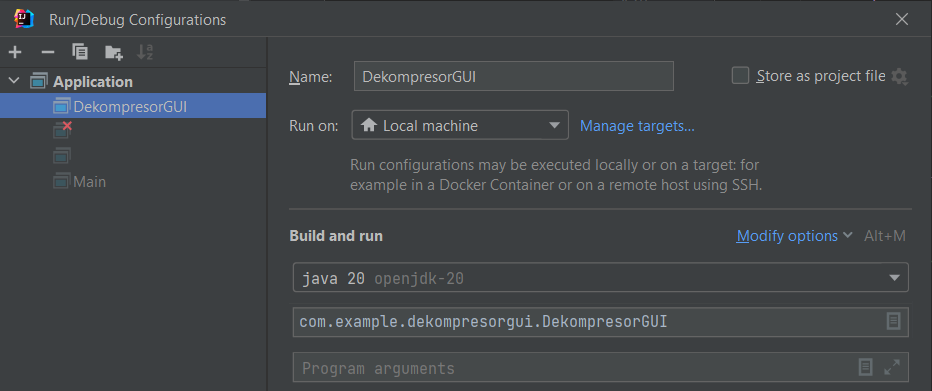
\includegraphics[width=\textwidth]{config1.png}
\newpage
\item
tryb wsadowy\\\\
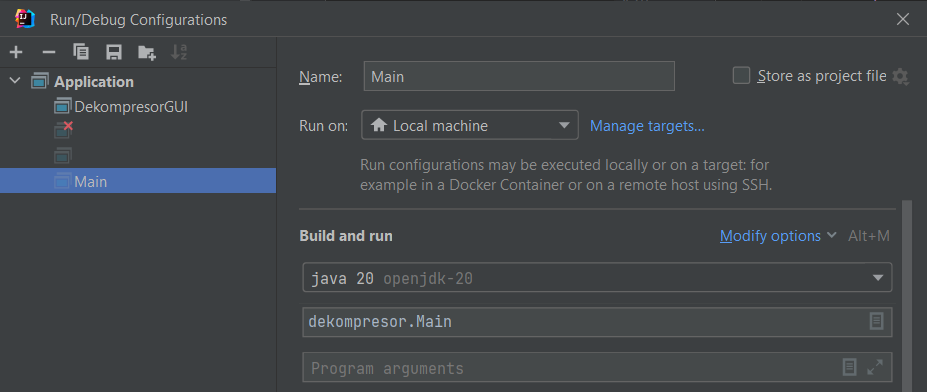
\includegraphics[width=\textwidth]{config2.png}
\end{itemize}
Ostatnim krokiem będzie dodanie biblioteki JavaFX do struktury projektu, co możemy zrobić poprzez przejście w File > Project Structure > Libraries. Następnie klikamy na '+' i odnajdujemy ścieżkę z JavaFX, który powinien być dołączony razem z projektem. Koniecznie wybieramy folder \textbf{lib}. Po wykonaniu tego zadania całość powinna się prezentować mniej więcej tak, jak na zrzucie poniżej:\\
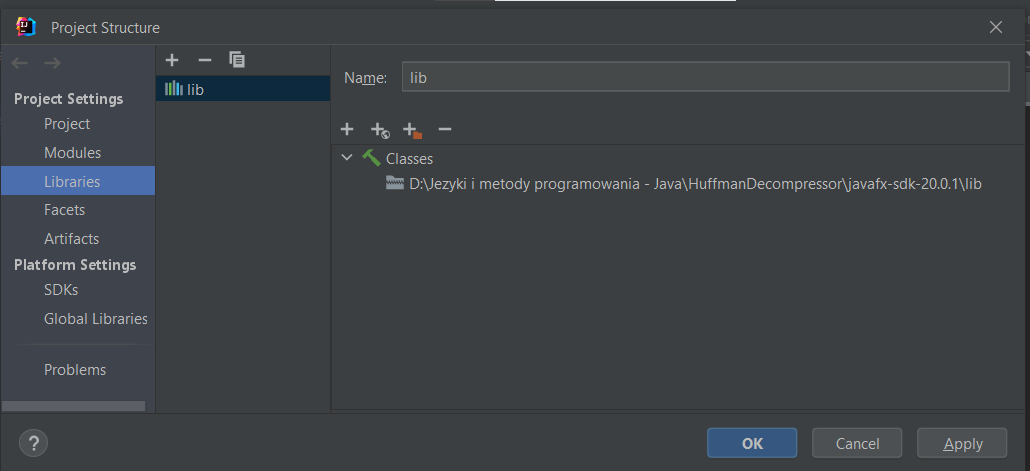
\includegraphics[width=\textwidth]{javafx.png}

\section{Przykłady wywołania programu}\label{header-n233}
Przedstawione zostały jedynie przykłady dla trybu wsadowego przy założeniu, że znajdujemy się w głównym katalogu projektu (w innym przypadku wymagane może być podanie innej ścieżki do pliku \textit{Dekompresor.jar})
\begin{itemize}
\item
\textbf{java -jar Dekompresor.jar test/8-bit/easy-text-test output}
\\Program wczyta plik o nazwie easy-text-test z katalogu test/8-bit i go zdekompresuje
\item
\textbf{java -jar Dekompresor.jar test/8-bit/cipher8 output -c}
\\Program wczyta plik o nazwie cipher8 z katalogu test/8-bit i zdekompresuje go do pliku output z włączonym szyfrowaniem używając domyślnego kodu "Politechnika\textunderscore Warszawska"
\item
\textbf{java -jar Dekompresor.jar -h}
\\Zostanie wyświetlona pomoc do programu
\end{itemize}
W przypadku trybu graficznego GUI jest bardzo przejrzyste i intuicyjne, jak widać na załączonym niżej zdjęciu oraz jego obsługa nie powinna sprawiać najmniejszych problemów. Składa się ono z następujących elementów:
\begin{itemize}
\item
przycisk do wyboru pliku, który chcemy zdekompresować
\item
pole tekstowe do wpisania względnej ścieżki pliku wyjściowego
\item
pola wyboru, w których możemy dostosować ustawienia
\item 
pole tekstowe do wpisania szyfru inny niż domyślny \textit{(dostępne jedynie po zaznaczeniu opcji szyfrowania)}
\item 
przycisk \textbf{\textit{Dekompresuj}} uruchamiający faktyczną część programu
\item 
pasek ładowania przedstawiający obecny stan dekompresji
\end{itemize}\\\\

\begin{center}
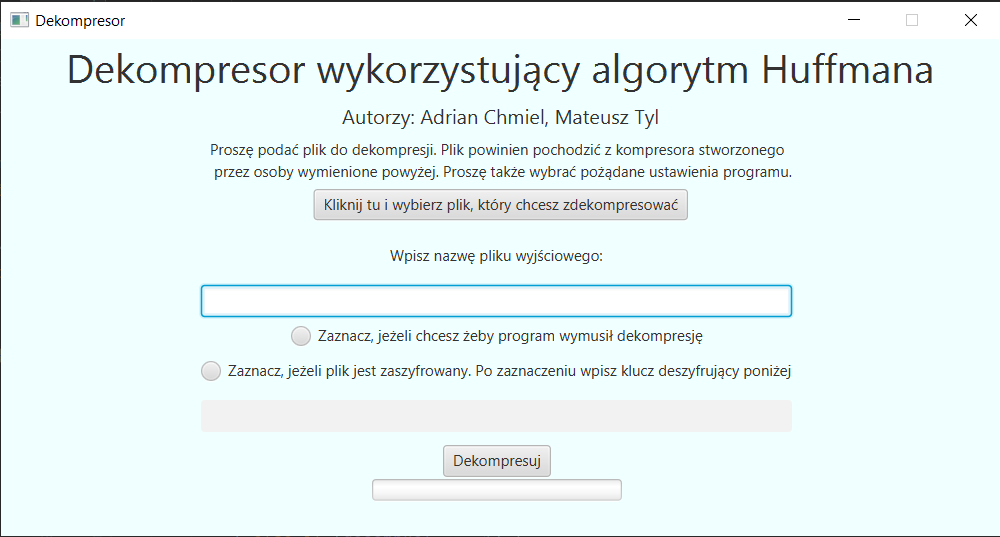
\includegraphics[width=0.95\textwidth]{dekompGUI.png}
\end{center}

\section{Wizualizacja słownika}\label{header-n233}
Wizualizacja słownika w postaci drzewa wyświetla się zaraz po ukończeniu dekompresji \textit{(lecz jedynie, gdy plik wejściowy został skompresowany 8-bitowo)}. Domyślnie jest mocno zbliżona do korzenia i zdecydowana większość drzewa może być niewidoczna na pierwszy rzut oka, dlatego zaimplementowana została możliwość przeciągania po okienku przy pomocy lewego klawisza myszy oraz przybliżania i oddalania widoku przy pomocy rolki.\\
Wizualizacja składa się z węzłów tj. kwadratów połączonych w odpowiedni sposób przy pomocy linii. Węzły zawierać mogą poszczególne dane:
\begin{itemize}
\item
kod odpowiadający danemu węzłowi znajdujący się bezpośrednio nad nim
\item
symbol odpowiadający danemu kodowi \textit{(jedynie, gdy jest to liść)}
\end{itemize}
Przykładowe zrzuty ekranu wizualizacji zawarte są poniżej:
\begin{itemize}
\item
Maksymalnie oddalony widok wizualizacji\\
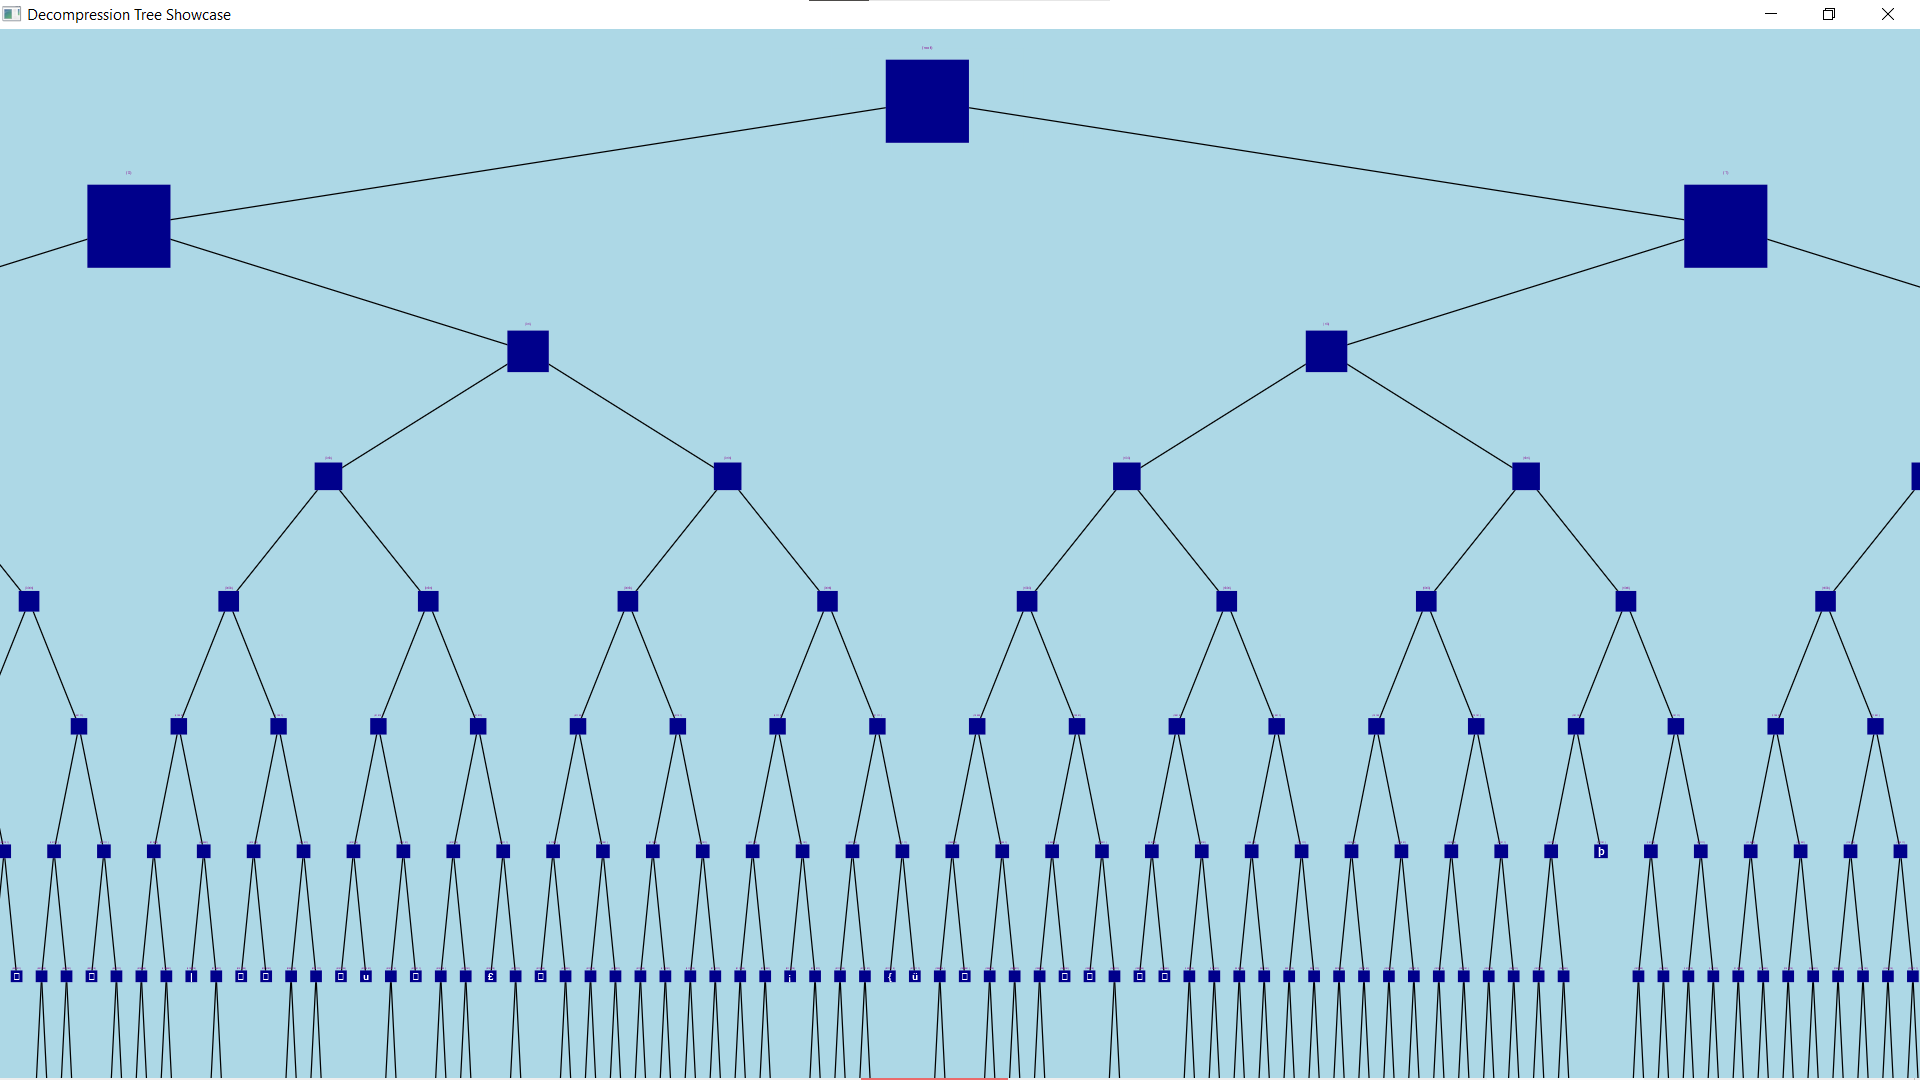
\includegraphics[width=\textwidth]{tree1.png}
\item
Zbliżenie na liście przedstawiające możliwość odczytania symboli i kodów\\
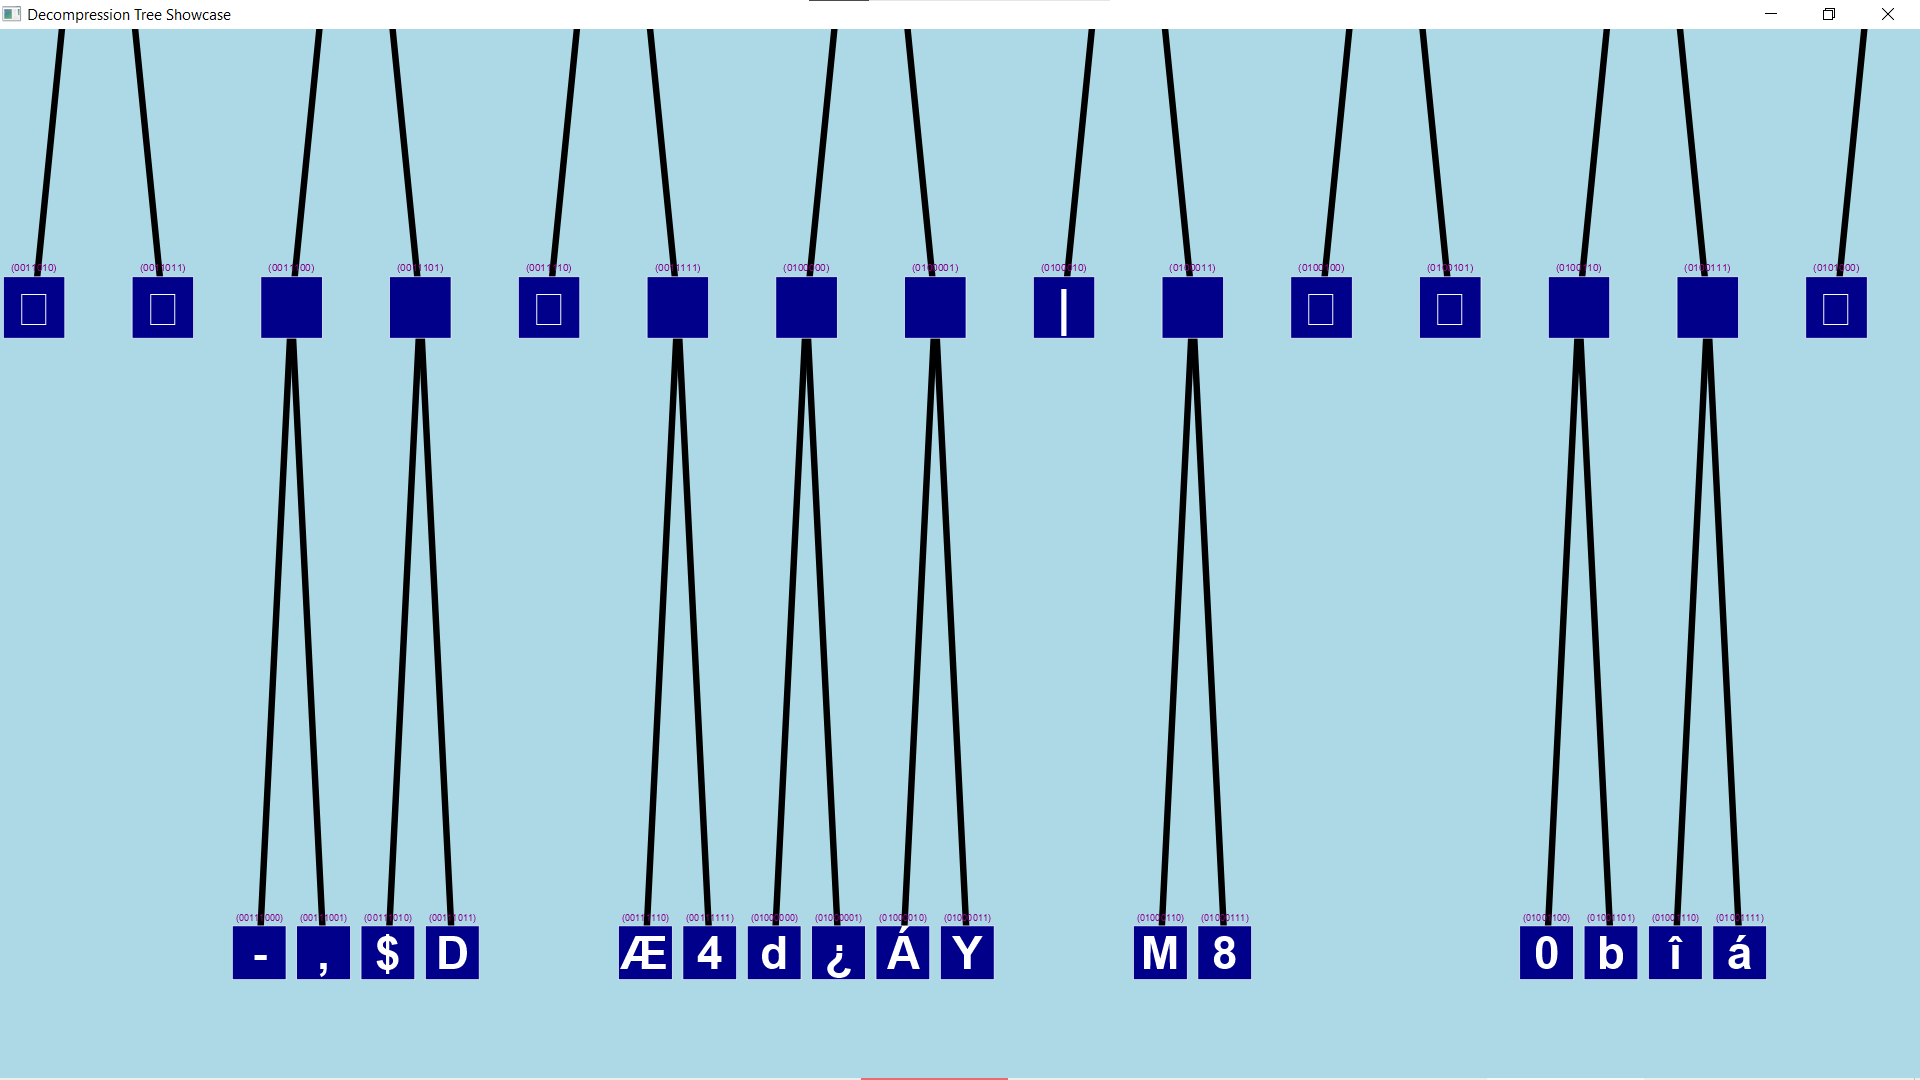
\includegraphics[width=\textwidth]{tree2.png}
\newpage
\item
Przykładowy fragment wizualizacji dla prostszego pliku\\
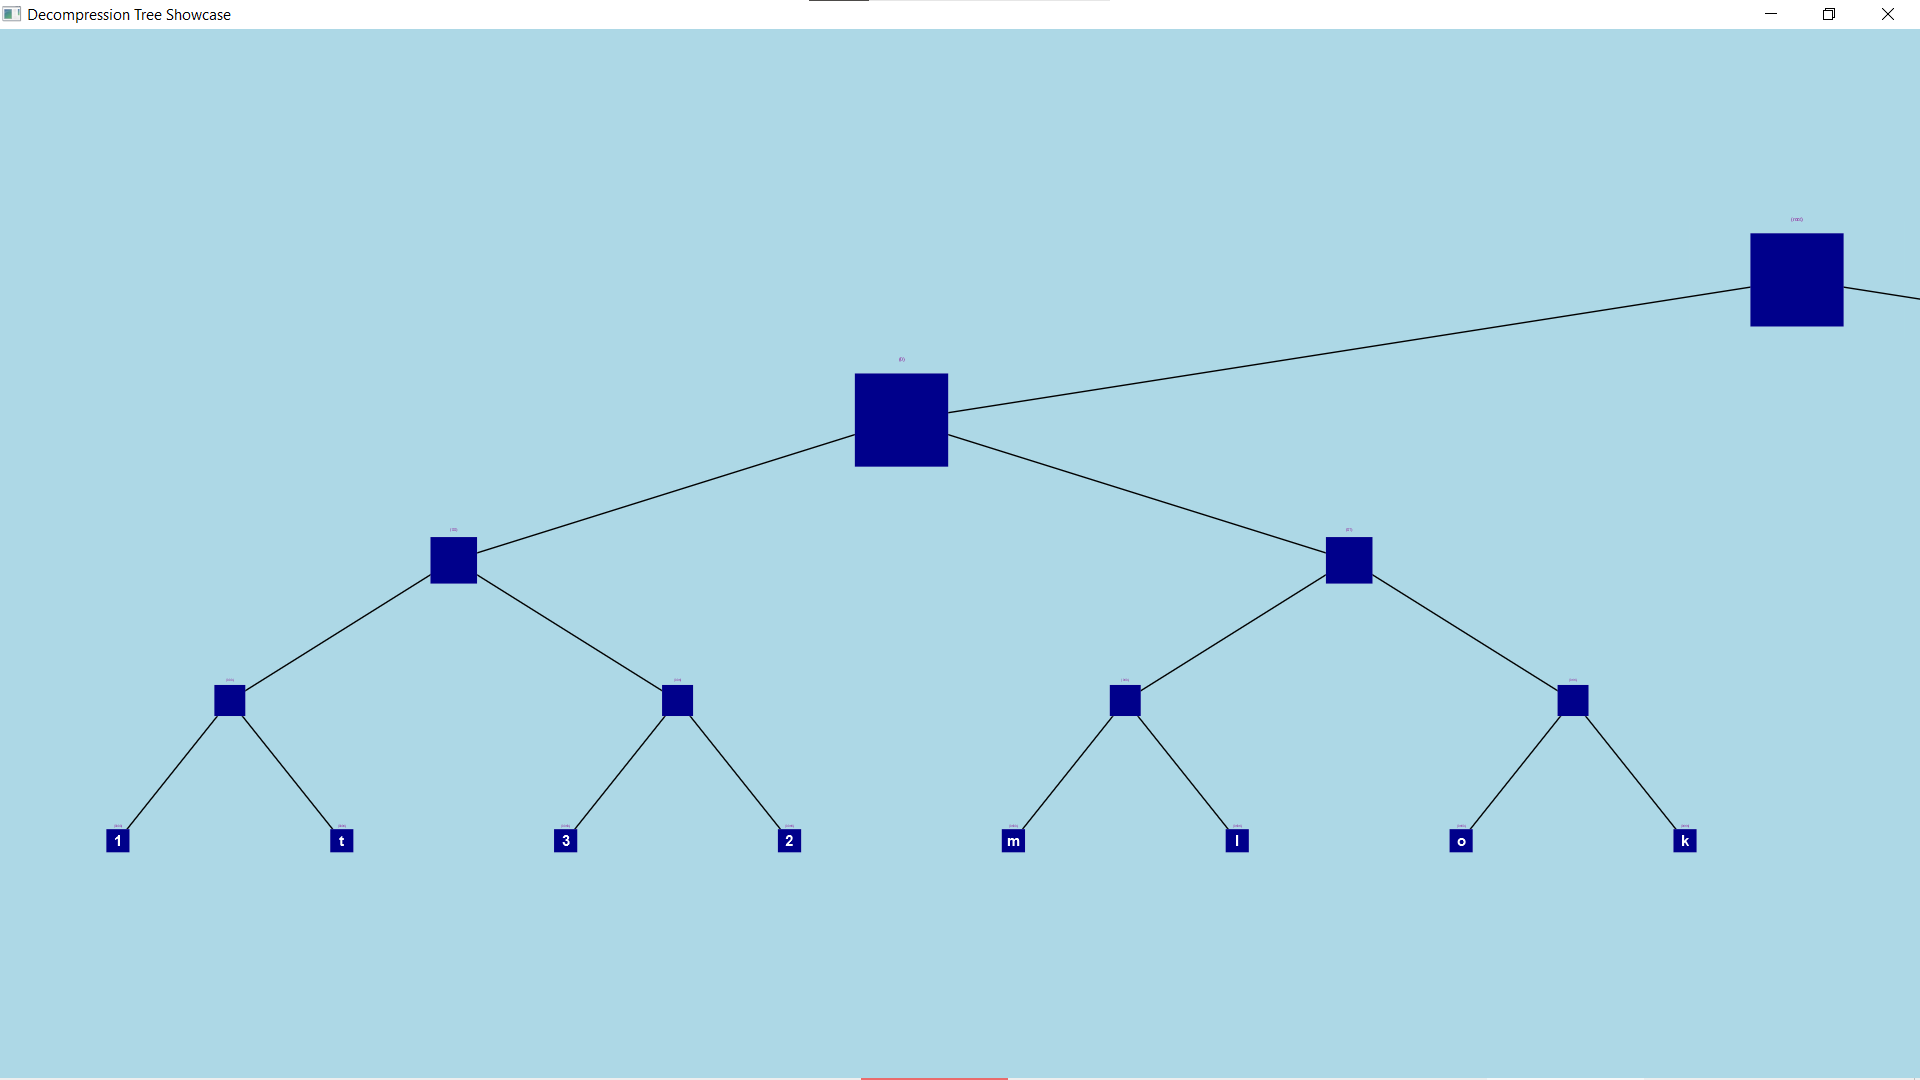
\includegraphics[width=\textwidth]{tree3.png}
\end{itemize}

\section{Struktura pliku wejściowego}\label{header-n279}
Pierwsze cztery bajty pliku wyjściowego zarezerwowane są na nagłówek. \\
Pierwsze dwa bajty nagłówka to pierwsze litery nazwisk autorów - CT.\\
Kolejny bajt to maska, z której można odczytać szczegółowe informacje o pliku. Ostatnim bajtem nagłówka jest wynik wyliczonej sumy kontrolnej.\\
Następnie pojawia się słownik, a na końcu znajdują się kolejno po sobie skompresowane dane w postaci kodów Huffmana o zmiennej długości.\\
W przypadku, gdy po zapisaniu wszystkich danych ilość bitów w ostatnim bajcie jest niekompletna, zostanie wykonane dopełnienie zerami. Jeżeli użytkownik wybierze zarówno brak kompresji, jak i brak szyfrowania, to otrzymuje on dokładnie ten sam plik, jak ten podany jako wejściowy.
\section{Struktura maski w nagłówku pliku}\label{header-n279}

    Szablon bitowy: 0bKKSZCEEE
\begin{itemize}
   \item K - sposób kompresji: 00 - brak, 01 - 8-bit, 10 - 12-bit, 11 - 16-bit
   \item  S - szyfrowanie: 0 - nie, 1 - tak
   \item  Z - zapisanie informacji, czy konieczne będzie usunięcie nadmiarowego znaku \textbackslash0 z końca pliku podczas dekompresji
   \item  C - dodatkowe sprawdzenie, czy ten plik jest skompresowany: 0 - nie, 1 - tak
   \item  E - ilość niezapisanych bitów kończących (tj. dopełniających ostatni bajt) zapisana binarnie
\end{itemize}
\section{Słownik}\label{header-n279}
Kod Huffmana każdego znaku wraz z odpowiadającym mu znakiem można odczytać ze słownika, który znajduje się od razu po nagłówku. Do odczytania słownika będzie potrzebny odpowiedni algorytm.\\
Algorytm prezentuje się następująco:\\
Tworzymy pomocnicze drzewo binarne. Rozpoczynamy analizę bitów składających się na słownik. Znajdujemy się w korzeniu drzewa. W zależności na co napotkamy analizując kolejne bity (analizujemy kolejno po dwa) robimy to co następuje:
\begin{itemize}
    \item 00 - przechodzimy po drzewie w dół do lewego syna, jeżeli ten jest nieodwiedzony, w przeciwnym razie do prawego syna
   \item  01 - to samo co 00, ale po tym przejściu znajdziemy się w liściu - wtedy otrzymujemy kod znaku w całości, kolejne 8/12/16 (w zależności od poziomu kompresji) bitów to znak, którego kod otrzymaliśmy.
   \item  10 - wycofanie się do ojca
   \item  11 - koniec słownika
\end{itemize}
W przypadku napotkania na 01 możemy z drzewa odczytać cały kod Huffmana dla konkretnego znaku. Kod czytamy od liścia w stronę korzenia. Z kolejnych 8/12/16 (w zależności od poziomu kompresji) bitów możemy odczytać kodowany znak. \\
\textbf{Uwaga - zawsze po odczytaniu znaku (tzn. odczytaniu 8/12/16 bitów) w drzewie należy wykonać cofnięcie z aktualnej pozycji do ojca!}
\\\\Przykład (dla kompresji 8 bitowej): \\
Nasz przykładowy słownik:
\begin{center}
\texttt{0101100010000001011001000101100001100101}
\end{center}
Analizujemy pierwsze dwa bity
\begin{center}
\texttt{\underline{01}01100010000001011001000101100001100101}
\end{center}
Zatem przechodzimy do lewego syna. Znajdujemy się w liściu, co oznacza że właśnie otrzymaliśmy znak. Odczytujemy z drzewa kod Huffmana dla aktualnego znaku. W tym przypadku jest to 0. Lewą gałąź w drzewie oznaczamy zerem, prawą jedynką.
Odczytujemy kolejne 8 bitów. Te bity to znak, którego kod Huffmana właśnie otrzymaliśmy.
\begin{center}
\texttt{01\underline{01100010}000001011001000101100001100101}
\end{center}
Otrzymaliśmy zatem pierwszy znak i odpowiadający mu kod Huffmana.\\
Znak w postaci binarnej: 01100010, w postaci dziesiętnej: 98\\
Odpowiadający mu kod Huffmana to: 0\\
Dalej postępujemy tak samo, pamiętając, że jeżeli napotkamy na \texttt{11} to słownik zostaje zakończony. W przypadku braku kompresji słownik nie jest wcale zapisywany.
 \section{Szyfrowanie}\label{header-n281} 
Szyfrowanie pliku odbywa się za pomocą \emph{Szyfrowania Vigenère’a}. Domyślnie kluczem szyfrowania jest: 
\texttt{Politechnika\textunderscore Warszawska} \\\\
W celu zmiany klucza szyfrowania możemy skorzystać z argumentu \texttt{-c "klucz"} np. \\
\texttt{-c "Huffman"} ustawi klucz szyfrowania na \texttt{Huffman} \\\\
Ten rodzaj szyfrowania polega na przesuwaniu kolejnych zapisywanych znaków o wartości ASCII kolejnych znaków znajdujących się w kluczu szyfrowania. W momencie, gdy podczas szyfrowania znajdziemy się na końcu klucza, należy po prostu wrócić na jego początek i kontynuować szyfrowanie przechodząc po nim kolejny raz. \\
Szyfrowaniu podlega słownik oraz skompresowany tekst, a więc wszystko oprócz nagłówka w postaci czterech pierwszych bajtów pliku.

\section{Struktura pliku wyjściowego}\label{header-n279}
Plikiem wyjściowym jest po prostu zdekompresowany plik, który jest identyczny z plikiem wcześniej skompresowanym przy użyciu kompresora naszego autorstwa w języku C.

\section{Komunikaty błędów}\label{header-n281}

\begin{enumerate}
\def\labelenumi{\arabic{enumi}.}
\item
Błąd podczas wczytywania pliku wejściowego: \texttt{Input file could not be opened!}
\item
Plik wejściowy jest pusty: \texttt{Input file is empty!}
\item
Błąd podczas wczytywania pliku wyjściowego:  \texttt{Output file could not be opened!}
\item
Pominięcie niezindentyfikowanych argumentów: \texttt{Unknown argument! (ignoring...)}
\item
Podany szyfr nie umożliwia pomyślnej dekompresji: \texttt{Decompression encryption failure!}
\item 
Napotkano błąd przy zapisie pliku wyjściowego: \texttt{Output file error!}
\item 
Napotkano błąd przy zapisie pliku pomocniczego do GUI: \texttt{Data file error!}
\item 
Napotkano błąd przy zapisie pliku realizującego wizualizację słownika: \texttt{Tree file error!}
\end{enumerate}

\section{Zwracane wartości}\label{header-n281}

Program po zakończeniu pracy zwraca wartość typu całkowitego, która może być użyteczna w przypadku identyfikacji różnego rodzaju niepowodzeń:

\begin{itemize}
\item
0 - Program zakończył się pomyślnie
\item
1 - Podano za mało argumentów
\item
2 - Błąd przy operacjach na pliku wejściowym
\item
3 - Błąd przy operacjach na pliku wyjściowym
\item
4 - Pusty plik wejściowy
\item
5 - Podano plik, który nie może zostać zdekompresowany
\item
6 - Podano nieprawidłowy szyfr przy dekompresji
\end{itemize}
Należy jednak pamiętać, że podanie nieprawidłowego szyfru może się również zakończyć powodzeniem, lecz uzyskany plik wynikowy nie będzie zgodny z oryginałem tj. plikiem przed kompresją.

\end{document}